\newpage 
\chapter{Linear Elliptic PDEs}
This chapter investigates the solvability of uniformly elliptic, second- order partial differential equations, subject to prescribed boundary condi- 
tions. We will exploit two essentially distinct techniques, energy methods 
within Sobolev spaces and maximum principle methods.

\section{Linear Elliptic PDEs}
Elliptic PDEs are a generalization of the Laplace equation 
\[
    -\Delta u = f. 
\]

\begin{definition}
[Symbol]
\label{def: Symbol}
The symbol of a partial differential operator is what we get when we replace $\partial_{j}$ with $i \xi_{j}$.
\end{definition}

It turns out that an important property is that $-\Delta = -\sum_{j} \partial_{j} \partial_{j}$ has (principal) symbol $-\sum_{j}\left(i \xi_{j}\right)^{2}=|\xi|^{2}$. What's important is that $|\xi|^{2}$ is nonzero and thus invertible for $\xi \neq 0$ :
$$
|\xi|^{2} \widehat{u}=\widehat{f} \Longrightarrow \widehat{u}=\frac{1}{|\xi|^{2}} \widehat{f} .
$$
This leads to the general definition of ellipticity of a partial differential operator.
Suppose that $P$ is a linear partial differential operator such that if $u=\left(u^{I}\right)_{I=1}^{N}: U \rightarrow$ $\mathbb{R}^{N}$, then $(P u)$ takes values in $\mathbb{R}^{N}$ and
$$
(P u)^{I}=\underbrace{\sum_{\substack{J, \alpha \\|\alpha|=K}} A_{J, \alpha_{1}, \ldots, \alpha_{d}}^{I} \partial^{\alpha} u^{J}}_{\text {principal part }}+(\text { lower order terms }) .
$$
Here, $K$ is called the \textbf{order} of $P$.

\begin{definition}
[Principal symbol]
\label{def: Principal symbol}
The principal symbol of an operator is
$$
\sigma_{\operatorname{prin}}(P)=i^{K} \sum_{\alpha=K} A_{J, \alpha_{1}, \ldots, \alpha_{d}}^{I}(x) \xi_{1}^{\alpha_{1}} \cdots \xi_{d}^{\alpha_{d}} .
$$
\end{definition}

Here, we allow the coefficients to be functions of $x$. We say that $P$ is \textbf{elliptic} if $\sigma_{\text {prin }}(P)$ is larger than $0$ for all $x \in U$ and $\xi \neq 0$.
The case $N=1$ is called the scalar case, where this looks like
$$
P u=\sum_{|\alpha|=K} a_{\alpha}(x) \partial^{\alpha} u
$$
Then the principal symbol is
$$
\sigma_{\text {prin }}(P)=i^{K} \sum_{\alpha} a_{\alpha}(x) \xi^{\alpha}
$$
The first nontrivial example is when $K=2$, so
$$
P u= - a^{i, j} \partial_{i} \partial_{j} u +b^{i} \partial_{i}u+c u.
$$
In this case, ellipticity is equivalent to $a^{i, j} \xi_{i} \xi_{j} \neq 0$ for all $x \in U$ and $\xi \neq 0$. This is equivalent to $a=\left[a^{i, j}\right]$ being a positive definite matrix for all $x \in U$.

We will assume that $a$ is a symmetric matrix and require the following property.

\begin{definition}
[Uniform ellipticity]
\label{def: Uniform ellipticity}
Uniform ellipticity is the property that there exists a uniform constant $\lambda>0$ such that $a^{i, j} \xi_{i} \xi_{j} \geq \lambda$ for all $x \in U$ and $|\xi|=1$.
\end{definition}

This is equivalent to saying that all eigenvalues of the matrix $a(x)$ are bounded below by $\lambda$.
Why do we care about elliptic PDEs?

\begin{itemize}
    \item These arise naturally in optimization problems in math, physics, etc. In the latter part of the course, we will discuss these in the context of calculus of variations.
    \item They also often arise as a part of evolutionary problems.
\end{itemize}

\begin{example}
[Incompressible Euler equations]
\label{eg: Incompressible Euler equations}
Let $u: \mathbb{R}_{t} \times \mathbb{R}^{3} \rightarrow \mathbb{R}^{3}$ represent the velocity of a fluid element at each point in time and space. This follows the equation
$$
\left\{\begin{array}{l}
\partial_{t}u + \cdot \nabla u+\nabla p=0 \\
\nabla \cdot u=0
\end{array}\right.
$$
This is one of the most infamous PDEs because of how difficult it is to understand. How do we figure out $p$ ? Take the divergence of the first equation to get that
$$
-\Delta p=\nabla(u \cdot \nabla u) .
$$
This is the \textbf{pressure equation}.
\end{example}

\newpage 
\section{Boundary Value Problems}
Assume $d \geq 2$ and $N=1$ (scalar case). Also assume uniform ellipticity of $P$ and some "nice" regularity for the coefficients $a, b, c$. We will focus mostly on the case where $U$ is a bounded domain in $\mathbb{R}^{d}$ with "nice" boundary.

When it comes to boundary value problems, you cannot prescribe both function values and values of the normal derivative at the boundary; this stems from the various uniqueness properties that arise for these PDEs. We will mostly focus on \textbf{Dirichlet boundary problems},
$$
\begin{cases}
    P u=f & \text { in } U 
    \\ u=g & \text { on } \partial U
\end{cases}
$$
We will focus less on boundary problems such as \textbf{Neumann boundary problems},
$$
\begin{cases}
    P u=f & \text { in } U \\ 
    \frac{\partial}{\partial \nu} u=g & \text { on } \partial U
\end{cases}
$$
We will study solvability for $u \in H^{1}(U)$. We will first study the Dirichlet boundary value problem $\left(\left.u\right|_{\partial u}=g\right.$ is okay due to the trace theorem). We will later discuss the Neumann boundary value problem, which needs to be studied in $H^{2}$ because we need to use the trace theorem on the derivative.

The standard reduction is that it suffices to understand $g=0$. This is because if we take any extension (with correct regularity) $\widetilde{g}: \bar{U} \rightarrow \mathbb{R}$ of $g$, then we can work with $v=u - \widetilde{g}$ and solve the problem
$$
\begin{cases}
    P v=f-P \widetilde{g}=\widetilde{f} & \text { in } U 
    \\ v=0 & \text { on } \partial U
\end{cases}
$$

\begin{definition}
[Divergence form]
\label{def: Divergence form}
$P$ is in divergence form if
$$
P u=-\partial_{j}\left(a^{i, j} \partial_{i} u\right)+ b^{i}\partial_i u +c u  .
$$
\end{definition}

Note that if $a$ is smooth, then
$$
Pu=a^{i, j} \partial_{i} \partial_{j}u+\left(\partial_{j} a^{i, j}+b^{i}\right) \partial_{i} u+cu. 
$$
We will see, however, that there are definite advantages to considering the two different representations of $ P $ separately. The divergence form is most natural for energy methods, based upon integration by parts , and the nondivergence form is most appropriate for maximum principle techniques. 

Our discussion of existence and uniqueness of the Dirichlet boundary value problem would be based on a-priori estimates. 

\begin{theorem}
[a-priori estimate]
\label{thm: a-priori estimate}
Suppose that $u \in H^{1}$ solves the Dirichlet boundary problem, and assume that $b, c \in L^{\infty}$ with $\|b\|_{L^{\infty}}+\|c\|_{L^{\infty}} \leq$ A. Then there exist constants $C>0$ and $\gamma \geq 0$ such that
$$
\|u\|_{H^{1}(U)} \leq C\|f\|_{H^{-1}}+\gamma\|u\|_{L^{2}(U)}
$$
\end{theorem}
\begin{proof}
The proof is essentially integration by parts. We can use approximation to justify the integration by parts. Write
\begin{align*}
       \int_{U}fu \, dx = \int_{U} P u ud x 
       &=\int_{U}\left(\partial_{i}\left(a^{i, j} \partial_{j} u+b^{i} u\right)+c u\right) u \,d x \\
        &=\int-a^{i, j} \partial_{j} u \partial_{i} u-b^{i} u \partial_{i} u+c u u \,d x
\end{align*}
Uniform ellipticity tells us that $\lambda|D u|^{2} \leq a^{i, j} \partial_{i} u \partial_{j} u$; integrate this to take care of the first term. The second term can be dealt with using Cauchy-Schwarz, and the third term is $\gamma\|u\|_{L^{2}}^{2} .$

Putting this all together gives
$$
\begin{aligned}
\lambda\|D u\|_{L^{2}(U)}^{2} & \leq C\|f\|_{H^{-1}}\|u\|_{H^{1}}+\int_{U}|b\|\partial u\| u| d x+\int_{U}|c||u|^{2} d x \\
& \leq C\|f\|_{H^{-1}}\|u\|_{H^{1}}+A \underbrace{\int_{U}|\partial u \| u| d x}_{\leq\|\partial u\|\|u\|_{L^{2}}}+A \underbrace{\int_{U}|u|^{2} d x}_{\leq \gamma\|u\|_{L^{2}}^{2}} .
\end{aligned}
$$
If we make $\gamma$ large enough so that we have put an $\|u\|_{L^{2}}^{2}$ on the right hand side and abosrb the second term, we get
$$
\|u\|_{H^{1}(U)}^{2} \leq C\|f\|_{H^{-1}}\|u\|_{H^{1}}+\gamma\|u\|_{L^{2}}\|u\|_{H^{1}} .
$$
\qed 
\end{proof}
\begin{remark}
We can alter this argument to only require $b\in L^{d+}$ and $c\in L^{d/2+}$.
\end{remark}

Recall that in order to prove existence statements with a priori estimates, we also needed to think about the dual problem for the adjoint $P^{*}$. (In finite dimensional linear algebra, $A x=y$ has a solution $x$ if and only if $r \in \operatorname{ran} A={ }^{\perp}\left(\operatorname{ker} A^{*}\right)$. For $P$ as above, let's compute $P^{*}$ with respect to $\langle u, v\rangle=\int u v d x$ :
$$
\int \partial_{j} u v d x=-\int u \partial_{j} v d x
$$
So
$$
P^{*}=-\partial_{j}\left(a^{j, k} \partial_{k} u\right)-\partial_{j}\left(b^{j} u\right)+c u,
$$
where we are assuming everything is real-valued. Note that the energy estimate also applies to $P^{*}$.

\subsection{Case 1: $P$ and $P^*$ Obey A-priori Estimates}
In our discussion of Sobolev spaces, we introduce Thm~\ref{thm: Uniqueness and Existence P} and Thm~\ref{thm: Uniqueness and Existence P*} from functional analysis. 

In our previous proof, we assumed that $X$ is reflexive to reduce (ii) to (i), but this assumption can be dropped. To see this argument, look for the "closed range theorem." The key idea is that $\overline{\operatorname{ran} P}=\perp^{\perp}\left(\operatorname{ker} P^{*}\right)$.

We want to apply this lemma to our $P, X=H_{0}^{1}$, and $Y=H^{-1}(U)$. In this setting, $X^{*}=H^{-1}(U)=Y$, and $Y^{*}=H_{0}^{1}(U)=X$.

In the energy estimate, we have an extra term $\gamma\|u\|_{L^{2}(U)}$ in the bound. For now, we will get rid of it by cheating. We will deal with it in full later. Here is when we have the energy estimate with $\gamma=0$ :

\begin{lemma}
\label{lem: Energy estimate gamma=0}
If $b=0$ and $c=0$, i.e. $P u=-\partial_{j}\left(a^{j, k} \partial_{j} u\right)$, then the energy estimate holds with $\gamma=0$.
\end{lemma}
\begin{proof}
    Proof. By density, $u \in C_{0}^{\infty}$.
    $$
    \begin{aligned}
    \int_{U} P u u d x &=\int_{U}-\partial_{j}\left(a^{j, k} \partial_{k} u\right) u d x \\
    &=\int_{U} a^{j, k} \partial_{j} u \partial_{k} u d x \\
    &\geq \lambda \int|D u|^{2} d x
    \end{aligned}
    $$
    Using Thm~\ref{thm: Friedrich inequality},
    $$
    \geq C \int_{U}|u|^{2} d x .
    $$
    As in the proof of the energy estimate, we cancel a factor of $\|u\|_{H^{1}}$ on both sides of the inequality to get the result.
    \qed 
\end{proof}
\begin{theorem}
\label{thm: Well-posedness gamma=0}
For every $f \in H^{-1}(U)$, there exixsts a unique $u \in H_{0}^{1}(U)$ such that $-\partial_{j}\left(a^{j, k} \partial_{j} u\right)=f$ in $U$.
\end{theorem}
\begin{remark}
\begin{itemize}
    \item []
    \item Since $P^{*}$ has the same form with the same constants, this condition gives the energy estimate with $\gamma=0$ for $P^{*}$, as well.
    \item For the proof of this, Evans' textbook uses the Lax-Milgram lemma, but our lemma is actually stronger.
\end{itemize}
\end{remark}

\subsection{Case 2: General $P$}

To obtain stronger results for our general problem, we will develop tools which are specifically useful for this problem. In particular, we will discuss Fredholm theory.

Recall the notion of a compact operator $K: X \rightarrow Y$ from functional analysis: $K\left(\bar{B}_{X}\right)$ is compact, where $B_{X}=\{x \in X:\|x\|<1\}$.

\begin{lemma}
[Solvability with compact operator]
\label{lem: Solvability with compact operator}
\begin{itemize}
    \item []
    \item For $K:X\to Y$, $K$ is compact if and only if $K^*$ is compact. 
    \item (Solvability of $(I+K)x=y$): Let $K:X\to Y$ be compact, and let $T=I+K$. 
    \begin{itemize}
        \item $ker(I+K)$ is finite dimensional;
        \item There exists an $n_0\ge 1$ such that $\ker(I+K)^n = \ker(I+K)^{n_0}$ for $n\ge n_0$; 
        \item $ran(I+K)$ is closed, so $rank(I+K) = {}^{\perp} (\ker(I+K^*))$;
        \item $\dim \ker(I+K) = \dim \ker(I+K^*)$. 
    \end{itemize}
\end{itemize}
\end{lemma}
\begin{proof}[][Pfsk]
     For the proof when $X$ is a Hilbert space, see the appendix of Evans' textbook. What is the idea? Here is how to think about compact operators: Notice that if $A$ has $\operatorname{dim} \operatorname{ran} A<\infty$, then $A$ is compact. Also notice that if $K_{n} \rightarrow K$ in the operator norm topology on $\mathcal{L}(X, Y)$, then $K$ is compact. Combining these two facts tells us that the closure of the set of finite rank operators is a subset of the compact operators; in separable Hilbert spaces, this is what all compact operators look like.
\end{proof}
\begin{remark}
    The last part is the general equivalent of the fact that in finite dimensional linear algebra, the row rank of a matrix is equal to the column rank of a matrix. This statement is that index $(I+K)=0$, where the index of an operator is the difference of these two quantities. The index tends to be very stable under perturbation.
\end{remark}

Why is this lemma relevant for us? Take any general
$$
P u=-\partial_{j}\left(a^{j, k} \partial_{k} u\right)+\partial_j(b_j u)+c u .
$$
In general, the energy estimate gives
$$
\|u\|_{H_{0}^{1}(U)} \leq C\|P u\|_{H^{-1}(U)}+\gamma\|u\|_{L^{2}(U)}
$$
But if we consider instead $(P+\mu I) u=-\partial_{j}\left(a^{j, k} \partial_{k} u\right)+\partial_j(b^{j} u)+(c+\mu) u$ with $\mu \gg 1$, then we can remove $\gamma$ on the right hand side.
Indeed,
$$
\int(P+\mu) u d x=\underbrace{\int-\partial_{j} a^{i, k} \partial_{k} u d x}_{\geq \lambda \int|D u|^{2} d x}+b, c \text { terms }+\int \mu u^{2} d x,
$$
where the $\int \mu u^{2} d x$ term is favorable if $\mu>0$. By case 1 , for $\mu$ sufficiently positive, for all $f \in H^{-1}$, ther exists a unique $u \in H_{0}^{1}$ such that
$$
(P+\mu I) u=f .
$$
We then have a well-defined map $(P+\mu I)^{-1}: H^{-1}(U) \rightarrow H_{0}^{1}(U)$. Now go back to
$$
(P+\mu) u-\mu u=P u=f
$$
Apply $(P+\mu)^{-1}$ to get
$$
u-\mu(P+\mu)^{-1} u=(P+\mu)^{-1} f .
$$
By Rellich-Kondrachov (recalling that $U$ is bounded), the embedding $\iota: H_{0}^{1}(U) \rightarrow L^{2}$ is compact. From this, it follows that
$$
(P+\mu)^{-1}: L^{2}(U) \rightarrow H^{-1}(U) \stackrel{(P+\mu)^{-1}}{\longrightarrow} H^{1}(U) \rightarrow L^{2}(U)
$$
is compact (since $A \circ K$ or $K \circ A$ is compact whenever $A$ is bounded and linear and $K$ is compact). Thus, $-\mu(P+\mu)^{-1}: L^{2}(U) \rightarrow L^{2}(U)$ is compact. Thus, our repackaging of the problem,
$$
u-\mu(P+\mu)^{-1} u=(P+\mu)^{-1} f,
$$
is of the form $(I+K) x=y$.

\begin{theorem}
[Fredholm alternative]
\label{thm: Fredholm alternative}
Let $P$ be as before, and let $U$ be a bounded domain with $C^{1}$ boundary.
\begin{itemize}
    \item[(i)] Exactly one of the following holds: 
    \begin{itemize}
        \item[(a)] (Solvability) For all $f \in H^{-1}(U)$, there exists a unique $u \in H_{0}^{1}(U)$ such that $P u=f$, and there exists a $C>0$ independent of $u, f$ such that $\|u\|_{H^{1}(U)} \leq$ $C\|f\|_{H^{-1}(U)}$.
        \item[(b)] (Existence of nonzero homogeneous solution) There exists a nonzero $u \in H_{0}^{1}(U)$ (or equivalently in $\left.L^{2}(U)\right)$ such that $P u=0$.
    \end{itemize}
    \item[(ii)] If (b) holds, then $\operatorname{dim} \operatorname{ker} P<\infty$ and $\operatorname{dim} \operatorname{ker} P^{*}<\infty$. Given $f \in H^{-1}(U)$, there exists a $u \in H_{0}^{1}(U)$ such that $P u=f$ if and only if $\langle f, v\rangle=0$ for all $v \in \operatorname{ker} P^{*}$.
\end{itemize}
\end{theorem}

\begin{remark}
\begin{itemize}
    \item []
    \item While our initial approach didn't really care about boundedness, this approach essentially relies on this condition.
    \item Part (ii) is a statement about norms. This will be an exercise and follows from compactness.
    \item  Here is a very nice consequence of this theorem. Take
    $$
    \widetilde{P} u=-\partial_{j}\left(a^{j, k} \partial_{k} u\right)+b^{j} \partial_{j} u .
    $$
    There is a weak maximum principle which says that
    $$
    \sup _{\bar{U}}|u|=\sup _{\partial U}|u| .
    $$
    This gives uniqueness in this Dirichlet problem. Then the Fredholm alternative gives us solvability from the uniqueness. We will properly discuss this later, when we go over maximum principles.
\end{itemize}
\end{remark}

\newpage 
\section{$L^2$-based Interior Regularity}
Last time, we discussed solvability for elliptic PDEs. Now we will talk about the regularity of solutions to elliptic PDEs. Here is a prototypical example.

\begin{example}
[Poisson equation]
\label{eg: Poisson equation}
 Consider the Poisson equation $-\Delta u=f$ in $U$, where $f \in H^{k}(U)$ or 
 $$
 f\in C^{k, \alpha}=\left\{u \in C^{k}(U): \partial^{\alpha} u \in C^{0, \alpha}(U) \forall|\alpha|=k\right\}.
 $$
 The idea is that $u$ should be more regular than $f$ by order 2. Interior regularity says that for all $V \subseteq \subseteq U$ (notation meaning $V$ is bounded and $\bar{V} \subseteq U)$,
$$
\|u\|_{H^{k+2}(V)} \leq C\|f\|_{H^{k}(V)}+C\|u\|_{L^{2}(U)}
$$
Similarly,
$$
\|u\|_{C^{k+2, \alpha}(V)} \leq C\|f\|_{C^{k, \alpha}(V)}+C\|u\|_{L^{\infty}(U)} .
$$
In general, the constant $C$ can depend on the domain $V$.
\end{example}

The first of these statements is referred to as \textbf{$L^{2}$-based regularity theory}, and the second is referred to as \textbf{Schauder theory}. We will think about $L^{2}$-based regularity theory for now and discuss Schauder theory later.

For $L^{2}$-based regularity theory, the key idea is integration by parts (the energy method)\footnote{Fraydoun Rezakhanlou says that he is an analyst, a PDE-ist, and a probabilist. He is an analyst because he uses the Cauchy-Schwarz inequality, a probabilist because he uses Chebyshev's inequality, and a PDE-ist because he uses integration by parts.}. We will make a simplifying that $u \in H^{k+2}(V)$; this is not assuming everything because from this qualitative fact, we will derive a quantitative bound. This assumption allows us to commute the equation with derivatives. We have not said any assumptions about the boundary, which may seem like an issue with integration by parts, but this is why we are discussing interior regularity. We will solve this with a cutoff function.
Let $\zeta$ be a nonnegative, smooth cutoff function which equals 1 in $V$ and equals 0 near $\partial U$. Then (squaring $\zeta$ in anticipation of a nice $L^{2}$ trick),
$$
\begin{aligned}
\int_{U} f u \zeta^{2} d x &=\int_{U}-\Delta u u \zeta^{2} \\
&=\sum_{j=1}^{d} \int_{U} \underbrace{\partial_{j} u \partial_{j}\left(u \zeta^{2}\right)}_{\partial_{j} u \zeta^{2}+2 u \zeta \partial_{j} \zeta} d x
\end{aligned}
$$
Note that we have no boundary term in the integration by parts thanks to $\zeta$.
$$
=\sum_{j=1}^{d} \int\left(\partial_{j} u\right)^{2} \zeta^{2}+2 \partial_{j} u u \zeta \partial_{j} \zeta d x
$$
Rearrange this to get
$$
\int_{U}|D u|^{2} \zeta^{2} d x \leq\left|\int_{U} f u \zeta^{2} d x\right|+\underbrace{2\left|\int_{U} u \zeta D u \cdot D \zeta d x\right|}_{\leq 2\left(\int_{U}|D u|^{2} \zeta^{2}\right)^{1 / 2}\left(\int_{U} u^{2}|D \zeta|^{2} d x\right)^{1 / 2}}
$$
To control this right term, we use the AM-GM inequality $a b \leq \frac{a}{2}+\frac{b}{2}$. But we can weight this by $\sqrt{\varepsilon}$ on $a$ and $\frac{1}{\sqrt{\varepsilon}}$ on $b$ to get the inequality $a b \leq \varepsilon \frac{a^{2}}{2}+\frac{1}{\varepsilon} \frac{b^{2}}{2}$. This bounds
$$
2\left(\int_{U}|D u|^{2} \zeta^{2}\right)^{1 / 2}\left(\int_{U} u^{2}|D \zeta|^{2} d x\right)^{1 / 2} \leq \varepsilon \int_{U}|D u|^{2} \zeta^{2} d x+\frac{1}{\varepsilon} \int_{U} u^{2}|D \zeta|^{2} d x .
$$
Now set $\varepsilon=1 / 2$ to absorb the first term to the right hand side. This gives
$$
\begin{aligned}
\frac{1}{2} \int_{U}|D u|^{2} \zeta^{2} d x & \leq\left|\int_{U} f u \zeta^{2}\right|+2 \int_{U} u^{2}|D \zeta|^{2} d x \\
& \leq\|f\|_{L^{2}(U)}+\|u\|_{L^{2}(U)},
\end{aligned}
$$
and we lower bound the left hand side by $\frac{1}{2} \int_{V}|D u|^{2} d x$. For the actual result, we could have upgraded the $\|f\|_{L^{2}(U)}$ to $\|f\|_{H^{1}(U)}$ by using an additional cutoff argument.
What about higher regularity? Suppose $k+2=2$. Then if $-\Delta u=f$, we get
$$
-\Delta \partial_{j} u=\partial_{j} f,
$$
where $\partial_{j} u \in H^{1}$, so we can do integration by parts. Now apply the case $k=1$ to get
$$
\int_{V}\left|D \partial_{j} u\right|^{2} d x \leq\left|\int_{U} \partial_{j} f \partial_{j} u \zeta^{2} d x\right|+\left\|\partial_{j} u\right\|_{L^{2}(U)}
$$
Bound the first term by (using the same AM-GM trick)
$$
\left|\int_{U} f \partial_{j}^{2} u \zeta^{2} d x\right| \leq \frac{1}{4 \varepsilon} \int_{U} f^{2} \zeta^{2} d x+\varepsilon \int_{U}\left|\partial_{j} u\right|^{2} \zeta^{2} d x
$$
Absorb the second term to the right hand side to get
$$
\int_{U}\left|D \partial_{j} u\right|^{2} \zeta^{2} d x \leq C \int_{U} f^{2} d x+C\|D u\|_{L^{2}(U)}^{2} .
$$
We want to change the last term into $\|u\|_{L^{2}(U)}$. Our tool to do this is the $H^{1}$ bound we just proved. But this needs us to have a domain in the interior of $U$. However, note that if we define $V \subseteq \subseteq W \subseteq \subseteq U$, we can replace this term on the the right hand side by $C\|D u\|_{L^{2}(W)}$. Then we use the $H^{1}$ bound $\|D u\|_{L^{2}(W)} \leq\|f\|_{L^{2}(U)}+\|u\|_{L^{2}(U)}$. In conclusion, we get
$$
\left\|D \partial_{j} u\right\|_{L^{2}(V)} \leq C\|f\|_{L^{2}(U)}+C\|u\|_{L^{2}(U)}
$$
for all $j$. Combined with the $H^{1}$ bound, this gives the $H^{2}$ bound
$$
\|u\|_{H^{2}(V)} \leq C\|f\|_{L^{2}(U)}+C\|u\|_{L^{2}(U)} .
$$

For the full $L^{2}$-regularity theorem, we have an elliptic operator
$$
P u=-\partial_{j}\left(a^{j, k} \partial_{k} u\right)+b^{j} \partial_{j} u+c u,
$$
where $u: U \rightarrow \mathbb{R}$ and $U$ is an open subset of $\mathbb{R}^{d}$. We also assume $a(x) \succ \lambda I$ for some $\lambda>0$ for all $x \in U$. Also assume $a, b, c \in L^{\infty}(U)$ (although the natural assumption for $d \geq 3$ is actually $a \in L^{\infty}, b \in L^{d}, c \in L^{d / 2}$ ). For the $H^{2}$ bound, we also make the assumption that $\partial a \in L^{\infty}(U)$; this comes from the fact that if we want to commute the derivative as in the argument above, we must be able to deal with the derivative of the coefficients $a^{i, j}$.

\begin{theorem}
[$H^2$ elliptic regularity]
\label{thm: $H^2$ elliptic regularity}
 Let $u \in H^{1}(U)$ be a weak solution to $P u=f$ on $U$, and let $f \in L^{2}(U)$. Then for all $V \subseteq \subseteq U, u \in H^{2}(V)$, and
$$
\|u\|_{H^{2}(V)} \leq C\left(\|f\|_{L^{2}(U)}+\|u\|_{L^{2}(U)}\right) .
$$
\end{theorem}
The proof of this theorem is the same as the previous argument but with some minor adjustments. The main step is integration by parts. Formally,
$$
\begin{aligned}
\int_{U}-\partial_{j}\left(a^{j, k} \partial_{k} v\right) v \zeta^{2} d x &=\int_{U} a^{j, k} \partial_{k} v \partial_{j} v \zeta^{2} d x+\int_{U} a^{j, k} \partial_{k} v v \zeta \partial_{j} \zeta d x \\
& \geq \lambda \int_{U}|D u|^{2} \zeta^{2} d x-\|a\|_{L^{\infty}} \cdot \underbrace{\int|D u| \zeta|v||D \zeta| d x}_{\leq \frac{\lambda}{2 \|a\|_{L^{\infty}}}|D v|^{2} \zeta^{2}+\frac{1}{\lambda}\|a\|_{L}^{\infty}|v|^{2}|D \zeta|^{2}}\\ 
&\geq \frac{\lambda}{2} \int_{U}|D v|^{2} \zeta^{2} d x-\frac{\|a\|_{L^{\infty}}^{2}}{\lambda} \int_{U}|v|^{2}|D \zeta|^{2} d x.
\end{aligned}
$$

Since we do not know a priori that $u \in H^{2}(V)$, need to modify the proof idea to commute the equation with difference quotients instead of derivatives.

\begin{definition}
[Difference quotient]
\label{def: Difference quotient}
 If $k \in\{1, \ldots, d\}$ and $h \in \mathbb{R} \backslash\{0\}$, the difference quotient is
$$
D_{k}^{h} v(x)=\frac{v(x+h e_k)-v(x)}{h}
$$
This converges to $\partial_{k} v(x)$ as $h \rightarrow 0$.
\end{definition}

\vspace{2em}
\begin{proof}[][Proof of Thm~\ref{thm: $H^2$ elliptic regularity}]
Here we only proof the case $k=0$. 

Step 0: Note that for $u \in H^{1}(U)$,
$$
P u=f \text { in } U \Longleftrightarrow\langle P u, \varphi\rangle=\langle f, \varphi\rangle \quad \forall \varphi \in C_{c}^{\infty}(U)
$$
Here, $P u \in H^{-1}(U), f \in L^{2} \subseteq H^{-1}$.
$$
\Longleftrightarrow\langle P u, \varphi\rangle=\langle f, \varphi\rangle \quad \forall \varphi \in H_{0}^{1}(U) \quad\left(=\left(H^{-1}(U)\right)^{*}\right)
$$
When we did our a priori estimate last time, we used approximation of $u$ by smooth functions. However, here, we want to show that we have extra regularity, so the equivalent of approximation is this step above.
$$
\Longleftrightarrow \int_{U} a^{j, k} \partial_{j} u \partial_{k} \varphi+b^{j} \partial_{j} u \varphi+c u \varphi d x=\int_{U} f \varphi d c \quad \forall \varphi \in H_{0}^{1}(U)
$$a


\noindent Step 1: Now commute the equation with $D_{j}^{h}$. Note that the Leibniz rule holds:
$$
D_{j}^{h}(u v)(x)=D_{j}^{h} u(x) v(x)+u(x+h) D_{j}^{h} v(x) .
$$
This comes from
$$
u v(x+h)-u v(x)=(u(x+h)-u(x)) v(x)+\underbrace{u(x+h)}_{=: u^{h}(x)}(v(x+h)-v(x)) .
$$
Now
$$
\begin{aligned}
D_{j}^{h} f &=D_{j}^{h}\left(-\partial_{j} a^{j, k} \partial_{k} u+b^{j} \partial_{j} u+c u\right) \\
&=-\partial_{\ell}\left(a^{h}\right)^{j, k} \partial_{k} D_{j}^{h} u+\left(b^{h}\right)^{j} \partial_{\ell} D_{j}^{h} u+c^{h} D_{j}^{h} u-\partial_{\ell}\left(D^{h} a\right)^{\ell, k} \partial_{k} u+\left(D_{j}^{h} b\right)^{\ell} \partial_{\ell} u+D_{j}^{h} c u .
\end{aligned}
$$
Rearrange this as
$$
-\partial_{\ell}\left(\left(a^{h}\right)^{\ell, k} \partial_{k} D_{j}^{h} u\right)=\widetilde{f}_{1}^{h}
$$
where $f_{1}^{h}$ is everything else. Now
$$
\left\langle-\partial_{\ell}\left(a^{h}\right)^{\ell, k} \partial_{k} D_{j}^{h} u, \varphi\right\rangle=\left\langle\widetilde{f}_{1}^{h}, \varphi\right\rangle \quad \forall \varphi \in H_{0}^{1}(U)
$$

where the left hand side equals
$$
\int\left(a^{h}\right)^{\ell, k} \partial_{k}\left(D_{j}^{h}\right) u \partial_{\ell} \varphi d x
$$

\noindent Step 2: " $\varphi=\partial_{j} u \zeta^{2 "}$ : Choose $\varphi=D_{j}^{h} \zeta^{2} \in H_{0}^{1}(U)$. By the integration by parts idea, we get
$$
\frac{\lambda}{2} \int_{U}\left|D D_{j}^{h} u\right|^{2} \zeta^{2} d x \leq \cdots \widetilde{f}_{1} D_{j}^{h} u
$$
One treats the right hand side like before, treating $D_{j}^{h} u$ like $\partial_{j} u$. To make this precise, we need the following lemma

\begin{lemma}
[Diffrence quotient to derivative]
\label{lem: Diffrence quotient to derivative}
Let $V\subset \subset U$. 
\begin{itemize}
    \item If $u \in W^{1, p},\left\|D_{j}^{h} u\right\|_{L^{p}(V)} \leq C\left\|\partial_{j} u\right\|_{L^{p}(U)}$ for $|h| \ll 1$. 
    \item     Assume $u \in L^{p}$. For $h \ll 1$, if $\| D_{j}^{h} u \|_{ L^{p}(V)} \leq A$, then $\partial_{j}u \in L^{p}$, and $\left\|\partial_{j} u\right\|_{L^{p}(V)} \leq A$.
\end{itemize}
\end{lemma}


This finishes the proof. 
\qed 
\end{proof}


%────────────────────────────────────────
\begin{remark}
 The constant $C$ is independent of $u$ and $f$ but dependent on $\lambda, \Lambda, V, U$.
The basic ideas in the proof were:
\begin{itemize}
    \item Integration by parts and ellipticity give us control over the highest order term.
    \item Commute the equation with $\partial_{j}$.
\end{itemize} 


In the proof, we looked at the equation for $\partial_{j} u$, then applied ellipticity to control $\left\|\zeta D \partial_{j} u\right\|_{L^{2}}$, where $\zeta$ was a smooth curoff which equals 1 on $B$ but is 0 near $\partial U$. In reality, however, to deduce that $u \in H^{2}(V)$, we have to work with the difference quotient $D_{j}(u)=\frac{u\left(x+h e_{j}\right)-u(x)}{h} .$
\end{remark}
%────────────────────────────────────────

Here is the higher regularity version of this theorem.


%────────────────────────────────────────
\begin{theorem}
[$H^k$ elliptic interior regularity]
\label{thm: $H^k$ elliptic interior regularity}
Assume the same hypotheses as before except 
\begin{itemize}
    \item $\left|D^{\alpha} a\right| \leq \text { A for all }|\alpha| \leq k-1,\left|D^{\alpha} b\right|+\left|D^{\alpha} c\right| \leq \text { A for all }|\alpha| \leq k-2 \text {, }$ 
    \item $f\in H^{k-2}(U)$. 
\end{itemize}
Then for all $V \subseteq \subseteq U, u \in H^{k}(V)$, and
$$
\|u\|_{H^{k}(V)} \leq C\left(\|f\|_{H^{k-2}(U)}+\|u\|_{L^{2}(U)}\right) .
$$
\end{theorem}
%────────────────────────────────────────

%────────────────────────────────────────
\begin{proof}[Pfsk of Higher orders]
 Here is a sketch. The proof follows the same idea, except we commute $D^{\beta}$ for $|\beta| \leq k-1$. Then look at the equation for $D^{\beta} u$ :
$$
\begin{aligned}
D^{\beta} f&=D^{\beta}(P u)\\ 
&=D^{\beta}\left(-\partial_{j}\left(a^{j, k} \partial_{k} u\right)+b^{j} \partial_{j} u+c u\right) \\
&=-\partial_{j}\left(a^{j, k} \partial_{k} D^{\beta} u\right)+D^{\beta}\left(b^{j} \partial_{j} u\right)+D^{\beta}(c u)
\end{aligned}
$$
Multiply both sides by $\zeta^{2} D^{\beta} u$. The first term on the right is
$$
\sum a^{j,k} \partial_k D^\beta u \partial_j D^\beta u \zeta^2 
$$
This gives us control of $\left\|D D^{\beta} u \zeta\right\|_{L^{2}(U)}$. For the rest of the terms, you do not see more than $k-1$ derivatives of of $u$ and $k-2$ derivatives of $b$ and $c$ after integration by parts.
In reality, the details need to be carried out with difference quotients, using induction to take care of lower derivative terms. The full proof is in Evans' book.
\qed
\end{proof}
%────────────────────────────────────────




%────────────────────────────────────────────────────────────────────────────────
\newpage
\section{$L^2$-based Boundary Regularity}
%────────────────────────────────────────────────────────────────────────────────
Previously, we have been looking at regularity away from the boundary. You may also notice that we have not been putting conditions on boundary behavior of $u$ (we only required, for example, $u \in H^{1}$ rather than $u \in H_{0}^{1}$ ).


%────────────────────────────────────────
\begin{theorem}
[$L^2$-based boundary regularity]
\label{thm: L^2-based boundary regularity}
Assume the same hypotheses as in the $H^{2}$ interior regularity theorem, except:
\begin{itemize}
    \item $u \in H_{0}^{1}(U)$ (i.e. $\left.u\right|_{\partial U}=0$ in the sense of traces).
    \item $\partial U$ is $C^{2}$.
\end{itemize}
Then $u \in H^{2}(U)$, and
$$
\|u\|_{H^{2}(U)} \leq C\left(\|f\|_{L^{2}(U)}+\|u\|_{L^{2}(U)}\right)
$$
\end{theorem}
%────────────────────────────────────────
%────────────────────────────────────────
\begin{proof}
 Assume for simplicity that $u \in H^{2}(U)$; we can take care of this by doing the argument with difference quotients instead of derivatives. We will omit the contribution of $b$ and $c$ because they do not contribute much, as we have seen. Start with the equation
$$
f=\partial_{j}\left(a^{j, k} \partial_{k} u\right)+\cdots .
$$
We want to take a derivative to say
$$
\partial_{\ell} f=-\partial_{\ell}\left(\partial_{j}\left(a^{j, k} \partial_{k} u\right)\right)
$$
but we cannot necessarily take the derivative at the boundary. However, notice that if the boundary is flat (wlog $\left\{x^{d}=0\right\}$ ), then all $\partial_{\ell}$ exist for $\ell=1, \ldots, d-1$. The only problem is the normal derivative $\partial_{x^{d}}=-\nu$. In other words only $(d-1)$-many directions (tangential to $\partial U$ ) are admissible.

For the sake of simplicity, take the special case when $U=B_{1}(0) \cap \mathbb{R}_{+}^{d}$ and supp $u \subseteq$ $B_{1 / 2}(0) \cap \mathbb{R}_{+}^{d}$.

%────────────────────────────────────────
\begin{figure}[H]
    \centering
    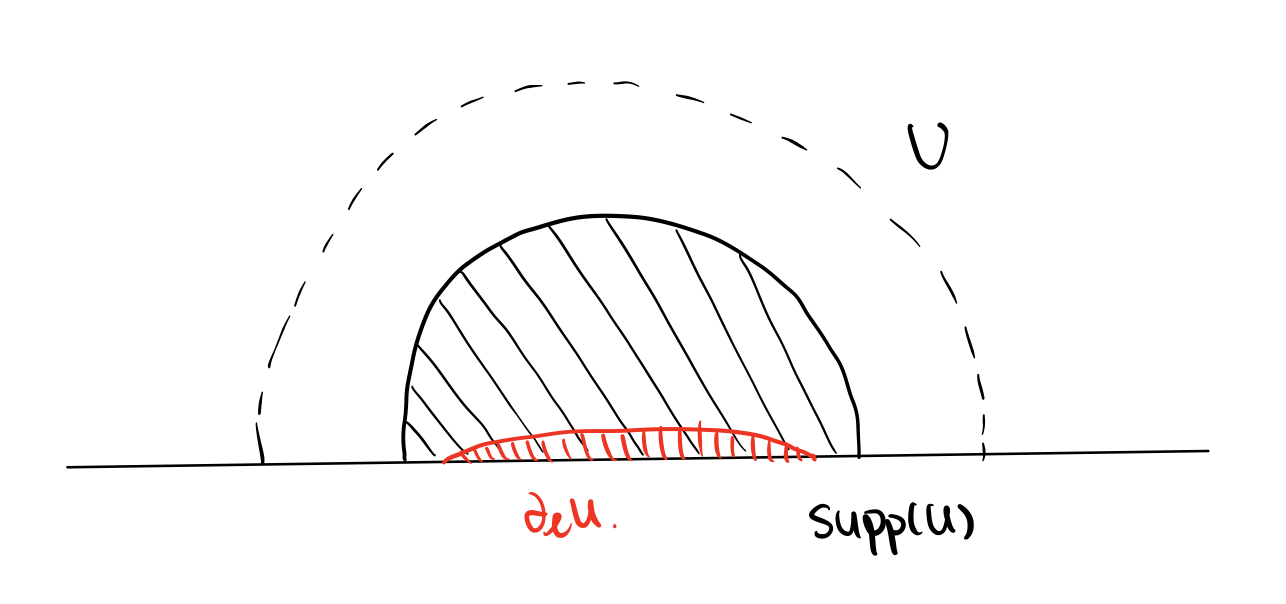
\includegraphics[width=0.7\textwidth]{figures/11-boundary.png}
\end{figure}
%────────────────────────────────────────

In this case, $\partial_l f=-\partial_{j}\left(a^{j, k} \partial_{k} \partial_{\ell} u\right)-\partial_{j}\left(\partial_{\ell} a^{j, k} \partial_{k} u\right)$ for $\ell=1, \ldots, d-1$. For these $d-1$ terms, we can use the cutoff $\zeta$ which equals 1 on $B_{1 / 2}(0)$ and is 0 near $\partial B_{1}(0)$ to get
$$
\left\|\zeta D \partial_{\ell} u\right\|_{L^{2}} \leq C\left(\|\zeta f\|_{L^{2}}+\|u\|_{L^{2}}\right) .
$$
In the integration by parts, there is an additional boundary term from $B_{1 / 2}(0) \cap\left\{x^{d}=0\right\}$. However, this contribution is zero because $\left.u\right|_{\partial U}=0$, which also implies $\left.\partial_{\ell} u\right|_{\partial U}=0$ for $\ell=1, \ldots, d-1$.

In this special case, it now remains to control $\left\|\zeta \partial_{x^{d}} \partial_{x^{d}} u\right\|_{L^{2}}$. The key observation is that the equation allows us to express $D_{\nu} D_{\nu} u$ in terms of everything else. Recall that the original equation is
$$
f=-\partial_{j}\left(a^{j, k} \partial_{k} u\right)+\cdots .
$$
The condition that $a \succ \lambda I$ is equivalent to $a^{j, k} \xi_{j} \xi_{k} \geq \lambda|\xi|^{2}$ for all $\xi \in \mathbb{R}^{d}$. If we take $\xi=e_{d}$, this tells us that $a^{d, d} \geq \lambda$. Now write the equation as
$$
f=\underbrace{-\partial_{d}\left(a^{d, d} \partial_{d} u\right)}_{=a^{d, d} \partial_{d}^{2} u-\left(\partial_{d} a^{d, d}\right) \partial_{d} u}-\sum_{\substack{j, k \\ j, k \neq d}} \partial_{j}\left(a^{j, k} \partial_{k} u\right) .
$$
We can divide the equation by $a^{d, d}$ to get
$$
\partial_{d}^{2} u=\frac{1}{-a_{d, d}}\left(a \cdot D_{\tan } u+(\partial a), b\right) D u+c u+f .
$$
This lets us control $\partial_{d}^{2} u$ by the other derivatives, completing the proof in this special case.
In general, we reduce to this special case by first using a smooth partition of unity and boundary straightening. In particular, for every $x \in \partial U$, there exists a ball $B_{r}(x)$ such that, after relabeling of the coordinate axes, $U \cap B_{r}(x)=\left\{x^{d}>\gamma\left(x^{1}, \ldots, x^{d-1}\right)\right\}$ for some $C^{2}$ function $\gamma$. We then take a boundary straightening map $y$, defined by
$$
\left\{\begin{array}{l}
y^{\ell}=x^{\ell} \\
y^{d}=x^{d}-\gamma\left(x^{1}, \ldots, x^{d}\right) .
\end{array} \quad \ell=1, \ldots, d-1\right.
$$
By compactness, $U \subseteq\left(\bigcup_{k=1}^{K} U_{k}\right) \cup U_{0}$, where $U_{k}$ are balls covering the boundary and $U_{0}$ contains the rest of the interior. Then there exists a smooth partition of unity $\left\{\chi_{k}\right\}_{k=0}^{K}$ subordinate to this cover, which gives
$$
u=\chi_{0} u+\sum_{k=1}^{K} \chi_{k} u
$$
The first term is supported on the interior of $U$, so we can apply our interior regularity theorem to it. For each other $\chi_{k} u$, when we change $x \mapsto y=y(x)$, we are reduced to the half-ball case already covered (both in terms of geometry and support of $u$ ). Check that the ellipticity constant of the resulting equation is still $\simeq \lambda$ and that $\partial \widetilde{a}(y), \tilde{b}(y)$ obey same bounds as before; this comes from writing the equation in terms of derivatives in $y$ and checking that the change of variables formula $a^{j, k}=\frac{\partial x^{j}}{\partial y^{j^{\prime}}} \widetilde{a}^{j^{\prime}, k^{\prime}} \frac{\partial x^{k}}{\partial y^{k^{\prime}}}$ preserves the $a \succ \lambda I$ condition. From the $H^{2}$ bound for $u_{k}(y)$, come back to $u \chi_{k}(x)$ (which needs the $C^{2}$ condition on $\left.\partial U\right)$.
\qed
\end{proof}
%────────────────────────────────────────

By compactness, $U \subseteq\left(\bigcup_{k=1}^{K} U_{k}\right) \cup U_{0}$, where $U_{k}$ are balls covering the boundary and $U_{0}$ contains the rest of the interior. Then there exists a smooth partition of unity $\left\{\chi_{k}\right\}_{k=0}^{K}$ subordinate to this cover, which gives
$$
u=\chi_{0} u+\sum_{k=1}^{K} \chi_{k} u
$$
The first term is supported on the interior of $U$, so we can apply our interior regularity theorem to it. For each other $\chi_{k} u$, when we change $x \mapsto y=y(x)$, we are reduced to the half-ball case already covered (both in terms of geometry and support of $u$ ). Check that the ellipticity constant of the resulting equation is still $\simeq \lambda$ and that $\partial \widetilde{a}(y), \tilde{b}(y)$ obey same bounds as before; this comes from writing the equation in terms of derivatives in $y$ and checking that the change of variables formula $a^{j, k}=\frac{\partial x^{j}}{\partial y^{j^{\prime}}} \widetilde{a}^{j^{\prime}, k^{\prime}} \frac{\partial x^{k}}{\partial y^{k^{\prime}}}$ preserves the $a \succ \lambda I$ condition. From the $H^{2}$ bound for $u_{k}(y)$, come back to $u \chi_{k}(x)$ (which needs the $C^{2}$ condition on $\left.\partial U\right)$.


%────────────────────────────────────────────────────────────────────────────────
\newpage
\section{Schauder Theory}
%────────────────────────────────────────────────────────────────────────────────

Schauder theory can be summarized as "H\"older-based elliptic regularity theory." Here are some of the main theorems.


%────────────────────────────────────────
\begin{theorem}
[Chaucer, interior regularity, divergence form]
\label{thm: Schauder, interior regularity, divergence form}
 Let $U$ be an open subset of $\mathbb{R}^{d}$, and suppose that $P u=f$, where $P u=-\partial_{j}\left(a^{j, k} \partial_{k} u\right), a \succ \lambda I$, and $a \in C^{k-1, \alpha}(\bar{U})$, Assume that $u \in C^{k, \alpha}(\bar{U})$ (with $k \geq 1$ and $\left.0<\alpha<1\right)$ and $f \in C^{k-2, \alpha}(\bar{U})$ (if $k=1$, we assume that $f=f^{0}+\sum_{j=1}^{d} \partial_{j} f^{j}$ with $\left.f^{0}, f^{j} \in C^{0, \alpha}(\bar{U})\right)$. Then for all $V \subseteq \subseteq U$, there exists a constant $C=C_{V}$ such that
$$
\|u\|_{C^{k, \alpha}(V)} \leq C\left(\|u\|_{L^\infty(U)}+\|f\|_{C^{k-2, \alpha}(U)}\right) .
$$
(If $k=1$, we define $\|f\|_{C^{-1, \alpha}}:=\left\|f^{0}\right\|_{C^{0, \alpha}}+\sum_{j=1}^{d}\left\|f^{j}\right\|_{C^{0, \alpha} .}$ )
\end{theorem}
%────────────────────────────────────────

%────────────────────────────────────────
\begin{remark}
We omit the $b^{j}+\partial_{j} u+c u$ parts because they can be easily added, and they are generally dealt with on a case-by-case basis to determine what regularity you need for $b$ and $c$.
\end{remark}
%────────────────────────────────────────


%────────────────────────────────────────
\begin{theorem}
[Schauder, interior regularity, non-divergence form]
\label{thm: Schauder, interior regularity, non-divergence form}
Let $U$ be an open subset of $\mathbb{R}^{d}$, and suppose that $Q u=f$, where $Q u=-a^{j, k} \partial_{j} \partial_{k} u, a \succ \lambda I$, and $a \in$ $C^{k-2, \alpha}(\bar{U})$, Assume that $u \in C^{k, \alpha}(\bar{U})$ (with $k \geq 2$ and $0<\alpha<1$ ) and $f \in C^{k-2, \alpha}(\bar{U})$. Then for all $V \subseteq \subseteq U$, there exists a constant $C=C_{V}$ such that
$$
\|u\|_{C^{k, \alpha}(V)} \leq C\left(\|u\|_{L^\infty(U)}+\|f\|_{C^{k-2, \alpha}(U)}\right) .
$$
\end{theorem}
%────────────────────────────────────────


%────────────────────────────────────────
\begin{definition}
[$C^{k,\alpha}$ boundary]
\label{def: C^{k,alpha} boundary}
Definition 12.1. We say that $U$ has $C^{k, \alpha}$ boundary if for all $x \in \partial U$, there exists an $r>0$ such that (after possibly rearranging the axes)
$$
U \cap B_{r}(x)=\left\{y \in B_{r}(x): y^{n}>\gamma\left(y^{1}, \ldots, y^{d-1}\right), \gamma \in C^{k, \alpha}\right\}
$$
\end{definition}
%────────────────────────────────────────


%────────────────────────────────────────
\begin{theorem}
[Schauder, boundary regularity, divergence form]
\label{thm: Schauder, boundary regularity, divergence form}
 Assume the same hypotheses in the interior divergence form theorem, and assume that $\partial U$ is $C^{k, \alpha}$ and $U$ is bounded. Take $P u=f$ with the boundary condition $\left.u\right|_{\partial U}=0$. Then there exists a constant $C$ such that
$$
\|u\|_{C^{k, \alpha}(U)} \leq C\left(\|u\|_{L^\infty(U)}+\|f\|_{C^{k-2, \alpha}(U)}\right) .
$$
\end{theorem}
%────────────────────────────────────────



%────────────────────────────────────────
\begin{theorem}
[Schauder, boundary regularity, non-divergence form]
\label{thm: Schauder, boundary regularity, non-divergence form}
Assume the same hypotheses in the interior divergence form theorem, and assume that $\partial U$ is $C^{k, \alpha}$ and $U$ is bounded. Take $P u=f$ with the boundary condition $\left.u\right|_{\partial U}=0$. Then there exists a constant $C$ such that
$$
\|u\|_{C^{k, \alpha}(U)} \leq C\left(\|u\|_{L^\infty(U)}+\|f\|_{C^{k-2, \alpha}(U)}\right) .
$$
\end{theorem}
%────────────────────────────────────────

Here are strategies to prove these theorems. 
\begin{itemize}
    \item []Interior:
    \begin{itemize}
        \item [] Step 1. Prove the result in the constant coefficient case ($a^{j,k}$ constant).
        \item [] Step 2.  Prove the general case using the constant coefficient case by the method of freezing the coefficients: Elliptic regularity is local, so we can split the space into small balls and prove the statement on each ball. The regularity of $a^{j,k}$ allows us to approximate the general problem by constant coefficient problems. 
    \end{itemize}
    \item [] Boundary:
    \begin{itemize}
        \item []     Step 0. Locally straighten the boundary to reduce to the case of half balls. 
        \item []    Step 1+2. Use the same method as for interior regularity. Step 0 makes the relevant constant coefficient problems be the half-space case.
    \end{itemize}
\end{itemize}
We will provide two proof for the constant coefficient case:
\begin{itemize}
    \item [A.] Littlewood-Paley theory proof. 
    \item [B.] Compactness + contradiction proof. 
\end{itemize}

%────────────────────────────────────────────────────────────────────────────────
\subsection{Littlewood-Paley Proof}

%────────────────────────────────────────
\begin{theorem}
[Constant coefficient Schauder estimate]
\label{thm: Constant coefficient Schauder estimate}
 Let $P u=-\partial_{j}\left(a_{0}^{j, k} \partial_{k} u\right)=$ $-a_{0}^{j, k} \partial_{j} \partial_{k} u$, where $a_{0}^{j, k}$ is constant on $\mathbb{R}^{d}$, and $a_{0} \succ \lambda I$. Assume that $\left|a_{0}^{j, k}\right| \leq \Lambda$, where $\Lambda \geq \lambda>0$. For $u \in C_{c}^{k, \alpha}\left(\mathbb{R}^{d}\right)$ and $f \in C^{k-2, \alpha}\left(\mathbb{R}^{d}\right)$ such that $P u=f$,
$$
\|u\|_{C^{k, \alpha}\left(\mathbb{R}^{d}\right)} \leq C\|f\|_{C^{k-2, \alpha}\left(\mathbb{R}^{d}\right)} .
$$
\end{theorem}
%────────────────────────────────────────
Let us emphasize that we assume that $u$ has compact support. We will focus on the case $k=2$.


%────────────────────────────────────────
\begin{definition}
[Little-Paley projection]
\label{def: Little-Paley projection}
Define 
$$
\begin{gathered}
\chi_{\leq 0}(\xi)= \begin{cases}1 & |\xi| \leq 1 \\
0 & |\xi|>1 \\
\geq 0 & \forall \xi\end{cases} \\
\chi_{\leq k}(\xi)=\chi_{\leq 0}\left(\xi / 2^{k}\right), \\
\chi_{k}(\xi)=\chi_{\leq k+1}(\xi)-\chi_{\leq k}(\xi) \quad\left(\text { so supp } \chi_{k} \subseteq\left\{\xi: 2^{k} \leq|\xi| \leq 2^{k+1}\right\}\right) .
\end{gathered}
$$
The Littlewood-Paley projections are 
\[
    P_{k} v=\mathcal{F}^{-1}\left(\chi_{k}(\xi) \widehat{v}\right), \quad P_{\leq k}v=\mathcal{F}^{-1}\left(\chi_{\leq k}(\xi) \widehat{v}\right).
\]
\end{definition}
%────────────────────────────────────────
Observe that for all $v \in \mathcal{S}^{\prime}\left(\mathbb{R}^{d}\right)$,
$$
v=P_{\leq k_{0}} v+\sum_{k>k_{0}} P_{k} v .
$$
If $v$ satisfies certain regularirt conditions in the same norm, $P_{\leq k_{0}} v \rightarrow 0$ as $k_{0} \rightarrow-\infty$. Note that $|\xi| \simeq 2^{k}$ on supp $\chi_{k}$.


%────────────────────────────────────────
\begin{lemma}
[Littlewood-Paley characterization of $C^{0,\alpha}(\RR^d)$]
\label{lem: Littlewood-Paley characterization of holder space}
Let $v \in C^{0, \alpha}\left(\mathbb{R}^{d}\right)$. Then
$$
[v]_{C^{0, \alpha}}=\sup _{\substack{x, y \\ x \neq y}} \frac{|v(x)-v(y)|}{|x-y|^{\alpha}} \simeq \sup _{k \in \mathbb{Z}} 2^{k \alpha}\left\|P_{k} v\right\|_{L^{\infty} .} .
$$
\end{lemma}
%────────────────────────────────────────
%────────────────────────────────────────
\begin{proof}
\begin{itemize}
    \item []
    \item Step 1: $\gtrsim$
    
    Both seminorms are invariant to scaling, so it suffices to consider $k=0$. So we just have to show that
$$
\left|P_{0} v\right| \lesssim[v]_{C^{0, \alpha}} .
$$
Since $\int \stackrel{\vee}{\chi}_{0}(y) d y=0$ iff $\chi_{0}(0)=0$,
\[
    \begin{aligned}
P_{0} v=\int \stackrel{\vee}{\chi}_{0}(x-y) v(y) d y &=\int \stackrel{\vee}{\chi}_{0}(x-y)(v(y)-v(x)) d y \\
& \leq \underbrace{\int \stackrel{\vee}{\chi}_{0}(x-y)|x-y|^{\alpha} d y}_{\text {fixed } \mathcal{S}\left(\mathbb{R}^{d}\right) \text { function }} [v]_{C^{0,\alpha}}.
\end{aligned}
\]
\item Step 2: $\lesssim$

Whenever we work with Littlewood-Paley theory, we should think about what scale we are working on. Let $L=|x-y|$, and choose $k_{0}$ so that $L^{-1} \simeq 2^{k_{0}}$. Decompose
$$
v(x)-v(y)=P_{\leq k_{0}} v(k)-P_{\leq k_{0}} v(y)+\sum_{k>k_{0}} P_{k} v(x)-P_{k} v(y)
$$
We can bound the latter two terms as
\begin{align*}
    \left\|\sum_{k \geq k_{0}} P_{\leq k_{0}} v\right\|_{L^{\infty}} &\leq \sum_{k<k_{0}}\left\|P_{k} v\right\|_{L^{\infty}}\\
&\leq \sum_{k \geq k_{0}} 2^{-k \alpha}[v]_{C^{0, \alpha}} \\
&\simeq L^{\alpha}[v]_{C^{0, \alpha}} .
\end{align*}
We can bound the first terms using the fundamental theorem of calculus:
$$
\begin{aligned}
\left|P_{\leq k_{0}} v(x)-P_{\leq k_{0}} v(y)\right| & \leq \| \nabla P_{\leq k_{0}} v \|_{L^{\infty} L} \\
& \leq \sum_{k \leq k_{0}}\left\|\nabla P_{k} v\right\|_{L^{\infty} L} \\
& \lesssim L \sum_{k \leq k_{0}} 2^{k} 2^{-k \alpha}[v]_{C^{0, \alpha}} \\
& \simeq L L^{-(1-\alpha)}[v]_{C^{0, \alpha}}
\end{aligned}
$$
\end{itemize}
\qed
\end{proof}
%────────────────────────────────────────

Now we can proof the theorem. 
\vspace{2em}
%────────────────────────────────────────
\begin{proof}[][Proof of Thm~\ref{thm: Constant coefficient Schauder estimate}]
    We have $P(P_k u) = P_k f$, so after fourier transform
    \[
        a^{j,l} \xi_j \xi_l \widehat{P_k u} = \widehat{P_k f}.
    \]
    Since $\lambda|\xi|^{2} \leq a_{0}^{j, \ell} \xi_{j} \xi_{k}$
$$
\widehat{P_{k} u}=\frac{2^{2 k}}{a^{j, \ell} \xi_{j} \xi_{\ell}} \widehat{P_{k} f} \widetilde{\chi}_{k} \frac{1}{2^{2 k}}=\frac{1}{2^{2 k}} \underbrace{\frac{2^{2 k}}{a^{j, \ell} \xi_{j} \xi_{\ell}}}_{\eta_{k}(\xi)} \tilde{\chi}_{k} \widehat{P_{k} f},
$$
where $\widetilde{\chi}_{k}=1$ on supp $\chi_{k}$ and $\operatorname{supp} \widetilde{\chi}_{k} \subseteq\left\{|\xi| \simeq 2^{k}\right\}$. Then
$$
P_{k} u=2^{-2 k} \eta_{k}^{\vee} * P_{k} f,
$$
SO
$$
\left\|P_{k} u\right\|_{L^{\infty}} \leq C 2^{-2 k}\left\|P_{k} f\right\|_{L^{\infty}} \leq C 2^{-2 k- k\alpha}[f]_{C^{0,\alpha}},
$$
which completes the proof. \footnote{Why?}
\qed
\end{proof}
%────────────────────────────────────────


\subsection{Compactness and Contradiction Proof}
%────────────────────────────────────────
\vspace{2em}
\begin{proof}[][Proof of Thm~\ref{thm: Constant coefficient Schauder estimate}]
    Here are the steps: 
    \begin{itemize}
        \item [1.] Assume that the desired inequality fails. Then there exist $a_{n}^{j, k}, u_{n}, f_{n}$ such that (after normalization)
        $$
        P_{n} u_{n}=f_{n}, \quad\left[u_{n}\right]_{C^{2, \alpha}}=1, \quad\left[f_{n}\right]_{C^{0, \alpha}} \leq \frac{1}{n} .
        $$
        After translation, we may also ensure that for some $\eta_{n} \in \mathbb{R}^{d}$,
        $$
        \left|D^{2} u_{n}\left(\eta_{n}\right)-D^{2} u_{n}(0)\right| \geq c\left|\eta_{n}\right|^{\alpha}
        $$
        Using scaling, we can assume that $\left|\eta_{n}\right|=1$.
        \item  
        Another massaging: Define $v_{n}(x)=u_{n}(x)-u_{n}(0)-x D u_{n}(0)-\frac{1}{2} x^{2} D^{2} u_{n}(0)$ to make $D^{2} v_{n}(0)=0$. Then
        $$
        P_{n} v_{n}=\tilde f_{n}, \quad \tilde{f}_{n} \rightarrow 0,\left[D^{2} v_{n}\right]_{C^{0, \alpha}}=1, \quad\left|D^{2} v_{n}\left(\eta_{j}\right)\right| \geq c .
        $$
        \item 
        Take the limit: Let $a_{n}^{j, k} \rightarrow a_{\infty}^{j, k}, \widehat{f}_{n} \rightarrow 0, v_{n} \rightarrow v$, and $\eta_{n} \rightarrow \eta_{\infty}$. Then $P_{\infty} v=0$ on $\mathbb{R}^{d}$, while
        $$
        \left[D^{2} v\right]_{C^{0, \alpha}} = 1, \quad D^{2} v\left(\eta_{\infty}\right) \neq 0
        $$
        But now use Liouville's theorem for $P_{\infty}$ (using Liouville's theorem for the Laplace equation) to get that $D^{2} v\left(\eta_{\infty}\right)=0$, a contradiction.
    \end{itemize}
\qed
\end{proof}
%────────────────────────────────────────



%────────────────────────────────────────────────────────────────────────────────
\newpage
\section{Maximum Principles}
%────────────────────────────────────────────────────────────────────────────────
Today, we will cover maximum principles. This material corresponds to section $6.5$ in Evans' textbook. This is a theory for solutions to elliptic PDEs in terms of their pointwise values (inherently scalar). Here, it is very important that $u: U \rightarrow \mathbb{R}$ is real-valued.

For today's lecture, it is more convenient to consider operators in non-divergence form:
$$
P u=-a^{j, k} \partial_{j} \partial_{k} u +b^{j} \partial_{j} u+c u .
$$
We assume the ellipticity condition, that $a \succ \lambda I$ for some $\lambda>0$, and we assume that $a, b, c \in L^{\infty}$. (Often, we will start with $c=0$.)

The theory of maximum principles should be thought of as a generalization of the theory of convex functions on $\mathbb{R}$. 

\subsection{The Weak Maximum Principle}

%────────────────────────────────────────
\begin{definition}
[(Classical) subsolution]
\label{def: (Classical) subsolution}
We say that $u\in C^2(U)$ is a classical subsolution if $Pu \le 0$. 
\end{definition}
%────────────────────────────────────────

%────────────────────────────────────────
\begin{remark}
When $d=1$ and $P=-a\partial_x^2$ with $a>0, Pu\le 0$ if and only if $u$ is convex. 
\end{remark}
%────────────────────────────────────────

%────────────────────────────────────────
\begin{theorem}
[Weak maximum principle]
\label{thm: Weak maximum principle}
 Let $U$ be a connected, bounded, open subset of $\mathbb{R}^{d}$. Let $u \in C^{2}(U) \cap C(\bar{U})$ with $P u \leq 0$. Assume for now that $c=0$. Then
$$
\max _{\bar{U}} u=\max _{\partial U} u \text {. }
$$
\end{theorem}
%────────────────────────────────────────
%────────────────────────────────────────
\begin{proof}
\begin{itemize}
    \item []
    \item Step 1: 

     Consider strict subsolutions $P u<0$. We will show that no interior maximum is possible. Suppose, for contradiction, that $x_{0} \in U$ is a (local) maximum. Then $D u\left(x_{0}\right)=0$, and the second derivative test tells us that $D^{2} u\left(x_{0}\right) \leq 0$. We have
    $$
    0>P u\left(x_{0}\right) = -\left.a^{j, k} \partial_{j} \partial_{k} u\right|_{x_{0}}+b^{j} \underbrace{\left.\partial_{j} u\right|_{x_{0}}}_{=D u=0}+\underbrace{c}_{=0} u = -\left.a^{j, k} \partial_{j} \partial_{k} u\right|_{x_{0}} = -tr(aD^2 u)|_{x_0}.
    $$
    Note that we can write 
    \[
        a = \sum_{i=1}^n \lambda_i v_i v_i^T. 
    \]
    Hence 
    \[
        -tr(aD^2 u) = - \sum_{i=1}^n \lambda_i \tr(v_iv_i^T D^2u) = - \sum_{i=1}^n \lambda_i v_i^T D^2u v_i.
    \]
    Therefore, we can find one direction such that $v_i^T D^2u v_i >0$, contradiction. 
    \item Step 2: 

    Upgrade to all subsolutions $u$. Introduce the approximation
    $$
    u_{\varepsilon}=u+\varepsilon v,
    $$
    where $v$ is a strict subsolution: $P v<0$ with $v \in C^{2}(U) \cap C(\bar{U})$. Then $u_{\varepsilon} \rightarrow u$ uniformly on $\bar{U}$, and
    $$
    P u_{\varepsilon}=P u+\varepsilon P v \leq \varepsilon P v<0 .
    $$
    How do we construct a strict subsolution $v$ ? We want something that is convex. A good candidate is $v=e^{x^{1}}$ because
    $$
    -a^{j, k} \partial_{j} \partial_{k}\left(e^{x^{1}}\right)=-a^{1,1} e^{x^{1}}<0
    $$
    We want to introduce a function which has a second order derivative much larger than a first order derivative. So instead consider $e^{\mu x^{1}}$, where $\mu$ is large. Then
    $$
    \begin{aligned}
    &-a^{j, k} \partial_{j} \partial_{k}\left(e^{\mu x^{1}}\right)=-a^{1,1} e^{\mu x^{1}} \leq-\lambda \mu^{2} e^{\mu x^{1}}, \\
    &\left|b^{j} \partial_{j} e^{\mu x^{1}}\right|=\left|-b^{j} \mu e^{\mu x^{1}}\right| \leq \sup |b| \cdot \mu e^{\mu x^{1}}
    \end{aligned}
    $$
    So if $\mu$ is large, $P v<0$.
\end{itemize}
\qed
\end{proof}
%────────────────────────────────────────


%────────────────────────────────────────
\begin{definition}
[(Classical) supersolution]
\label{def: (Classical) supersolution}
We say that $u\in C^2(U)$ is a classical supersolution if $Pu\ge 0$.
\end{definition}
%────────────────────────────────────────

Similarly, we have the following minimum principle.
%────────────────────────────────────────
\begin{theorem}
[Weak minimum principle]
\label{thm: Weak minimum principle}
 Have the same hypotheses except assume that $P u \geq 0$ and $c=0$. Then
$$
\min _{\bar{U}} u=\min _{\partial U} u
$$
\end{theorem}
%────────────────────────────────────────

%────────────────────────────────────────
\begin{remark}
$u$ is a solution if and only if it is a subsolution and a super solution. So under the same hypotheses with $P u=0$, we get
$$
\max _{\bar{U}}|u|=\max _{\partial U}|u|
$$
\end{remark}
%────────────────────────────────────────


%────────────────────────────────────────
\begin{corollary}
[Weak maximum principle, $c\ge 0$]
\label{thm: Weak maximum principle, cge0}
Suppose $U$ is a bounded, open connected subset of $\mathbb{R}^{d}$ and $u \in C^{2}(U) \cap C(\bar{U})$. For $P u \leq 0$.
$$
\begin{aligned}
&P u \leq 0 \Longrightarrow \max _{\bar{U}} u\leq \max _{\partial U} u^{+}, \\
&P u \geq 0 \Longrightarrow \min _{\bar{U}} u\leq \min _{\partial U} u^{-},
\end{aligned}
$$
where
$$
u^{+}=\left\{\begin{array}{ll}
u & \text { if } u>0 \\
0 & \text { if } u \leq 0,
\end{array} \quad u^{+}= \begin{cases}0 & \text { if } u \geq 0 \\
-u & \text { if } u<0\end{cases}\right.
$$
\end{corollary}
%────────────────────────────────────────
%────────────────────────────────────────
\begin{proof}
 Here is the max part: Let $V=\{x \in U: u(x)>0\}$, and let $Q u=P u-c u$. $Q$ satisfies the hypotheses and has no zero order term: $u \leq-c u \leq 0$ in $V$. The weak maximum principle for $Q$ on $V$ gives $\max _{\bar{V}} u \leq \max _{\partial V} u$. Note that the maximum of $u$ on $\partial V$ is the maximum of $u$ on $\partial U$. So we get the claim.
\qed
\end{proof}
%────────────────────────────────────────

We also have the comparison principle. 

%────────────────────────────────────────
\begin{theorem}
[Comparison principle]
\label{thm: Comparison principle}
 Let $U$ be an open, bounded, connected subset of $\mathbb{R}^{d}$. Let $P$ be elliptic with $c \geq 0$. Suppose $u, v \in C^{2}(U) \cap C(\bar{U})$ with $P u \leq 0$ in $U$ and $P v \geq 0$ in $U$. If $u \leq v$ on $\partial U$, then $u \leq v$ on $U$.
\end{theorem}
%────────────────────────────────────────

\subsection{The Strong Maximum Principle}

%────────────────────────────────────────
\begin{theorem}
[Strong maximum principle]
\label{thm: Strong maximum principle}
 Let $U$ be an open, bounded, connected subset of $\mathbb{R}^{d}$, and let $c=0$. Let $u \in C^{2}(U) \cap C(\bar{U})$ be such that $P u \leq 0$. If $u$ has a maximum at $x_{0} \in U$ (i.e.,$u(x)=\max _{\bar{U}} u$), then $u$ is constant on $U$.
\end{theorem}
%────────────────────────────────────────
Think of the picture of convex functions. The only way to have a maximum in the interior is if the whole function is constant (the graph is a horizontal straight line). Before, we prove this theorem, we need the following lemma.


%────────────────────────────────────────
\begin{theorem}
[Hopf's lemma]
 Let $U$ be an open, bounded, connected subset of $\mathbb{R}^{d}$ and $Pu\le 0$ in $U$. Suppose that $x_{0} \in \partial U$ is such that
 \begin{itemize}
     \item [(1)] there exists some $x_1\in U$ and $r_1>0$ such that $B_{r_1}(x_1) \subset U$, and $\overline{B_{r_1}(x_1)}\cap\partial U = \{x_0\}$,
     \item [(2)] $u(x_0)> u(x)$ in $\overline{B_{r_1}(x_1)}$, 
     \item [(3)] $u(x_0)> u(x)$ in $B_{r_1}(x_1)$. 
 \end{itemize}
 Then the normal derivative $\frac{\partial u}{\partial \nu}|_{x_0} >0$. 
\end{theorem}
%────────────────────────────────────────
\begin{proof}
Without loss of generality, take $x_{1}=0$. Consider $v=e^{-\mu|x|^{2}} - e^{-\mu r_1^2}$ so that $v(x)=0$ on $\left\{|x|=r_{1}\right\}$. Then $P v \le 0$ on $B_{r_{1}} \backslash B_{r_{1} / 2}$ for large $\mu$ (this is the same type of computation as before). Try to compare $u$ to $w=-\varepsilon v+u\left(x_{0}\right)$, where
$$
P w=-\varepsilon P v+P u\left(x_{0}\right)= -\varepsilon P v \geq 0 .
$$
%────────────────────────────────────────
\begin{figure}[H]
    \centering
    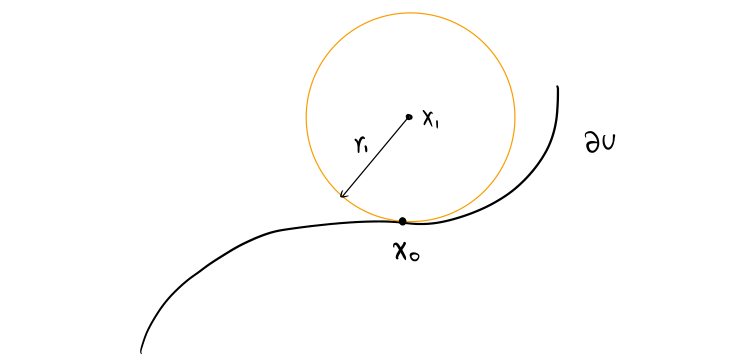
\includegraphics[width=0.8\textwidth]{figures/12-Hopf.png}
\end{figure}
%────────────────────────────────────────
Let $V=B_{r_{1}} \backslash B_{r_{1} / 2}$, so $\partial V=\partial B_{r_{1}} \cup \partial B_{r_{1} / 2}$. On the outer boundary $\partial B_{r_{1}}, w=u\left(x_{0}\right) \geq u$. On the inner boundary $\partial B_{r_{1} / 2}, w=-\varepsilon v+u\left(x_{0}\right)$. So for small enough $\varepsilon$, on the inner boundary, $u\left(x_{0}\right)>u(x)+\varepsilon v$. By the comparison principle, $w \geq u$ on $V=B_{r_{1}} \backslash B_{r_{1} / 2}$. Since 
\[
    u(x) + \varepsilon v - u(x_0)<0 , \quad u(x_0) + \varepsilon v(x_0) - u(x_0) = 0,
\]
we have 
\[
    \frac{\partial(u + \varepsilon v)}{\partial \nu}\Bigg|_{x_0} \ge 0 \Rightarrow  \frac{\partial u}{\partial \nu} \Bigg |_{x_0}\ge -\varepsilon \frac{\partial v}{\partial \nu} \Bigg|_{x_0} = 2\varepsilon r_1 e^{-\mu r_1^2}>0.
\]
\qed
\end{proof}
%────────────────────────────────────────

\vspace{2em}

%────────────────────────────────────────
\begin{proof}[][Proof of Thm~\ref{thm: Strong maximum principle}]
 Let $V=\{x \in U: u(x) \leq M\}$, where $M=\sup _{\bar{U}} u$. Then for $x_{0} \in U$, if $u\left(x_{0}\right)=M$, then $V \subsetneq U$. Assume for contradiction that $V \neq \varnothing$. Find a point $x_{1}$ closer to $\partial V$ than $\partial U$ and consider the biggest $r_{1}$ such that $B_{r_{1}}\left(x_{1}\right) \subseteq V$. Let $x_{0} \in B_{r_{1}}\left(x_{1}\right) \cap \partial V$. 
%────────────────────────────────────────
\begin{figure}[H]
    \centering
    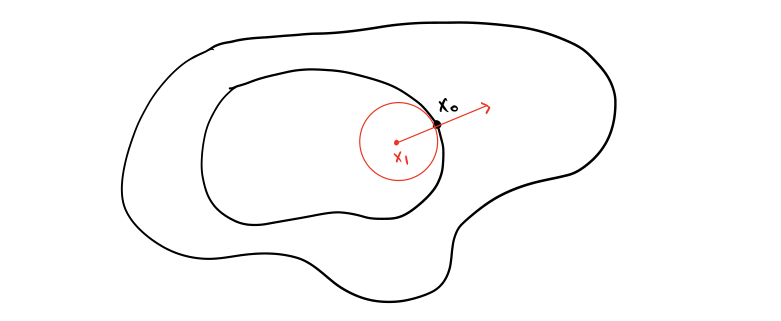
\includegraphics[width=0.8\textwidth]{figures/12-Strong-maximal.png}
\end{figure}
%────────────────────────────────────────
We may arrange, by taking $x_{1}$ close enough to $\partial V$, so that Hopf's lemma is applicable. This tells us that $\left.\frac{\partial}{\partial \nu} u\right|_{x=x_{0}} \neq 0$. But this contradicts the facr that $u\left(x_{0}^{\prime}\right)=M$ implies $\left.D u\right|_{x=x_{0}}=0$
\qed
\end{proof}
%────────────────────────────────────────

Similarly, we can prove the following strong maximum principle with $c\ge 0$: 

%────────────────────────────────────────
\begin{theorem}
[Strong maximum principle with $c\ge 0$]
\label{thm: Strong maximum principle with cge 0}
For $U$ being open, bounded and connected subset of $\mathbb{R}^{d}$, and $u \in C^{2}(U) \cap C(\bar{U}), c \geq 0$, then we have
\begin{itemize}
    \item If $Pu \le 0$ and $u$ has a nonnegative maximum at $x_0\in U$, then $u=$ const in $U$. 
    \item If $Pu \ge 0$ and $u$ has a nonpositive minimum at $x_0 \in U$, then $u=$ const in $U$. 
\end{itemize}
\end{theorem}
%────────────────────────────────────────



%────────────────────────────────────────────────────────────────────────────────
\newpage
\section{General Boundary Value Problems}
%────────────────────────────────────────────────────────────────────────────────

In this lecture, we will assume that $P$ is an elliptic operator in divergence form:
$$
P u=-\partial_{j}\left(a^{j, k} \partial_{k} u\right)+b^{j} \partial_{j} u+c u .
$$
Let $U$ be an open, bounded, connected subset of $\mathbb{R}^{d}$ with $C^{1}$ boundary $\partial U$. A general boundary value problem might be of the form
$$
\begin{cases}P u=0 & \text { in } U \\ \left.B u\right|_{\partial_{U}}=g & (\text { on } \partial U)\end{cases}
$$
for some operator $B$.
So far, we have focused on the Dirichlet boundary condition
$$
\begin{cases}P u=0 & \text { in } U \\ \left.u\right|_{\partial_{U}}=g & (\text { on } \partial U)\end{cases}
$$
By introducing an extension $\tilde{g}$ of $g$ to $U$, we could set, without loss of generality, $g=0$. With this reduction, the problem we have considered is
$$
\begin{cases}P u=0 & \text { in } U \\ \left.u\right|_{\partial_{U}}=0 & (\text { on } \partial U)\end{cases}
$$
Our goal now is to generalize our elliptic theory to other boundary conditions. This will force us to consider what is a "regular" boundary value problem for PDEs. In order to solve a $k$-th order ODE, you need $k$ pieces of data on the boundary. For the wave equation, which is a second order PDE, you impose boundary values and normal derivative values. Unlike ODEs, the wave equation, or Cauchy-Kovalevskaya, when we work with an elliptic PDE like $-\Delta u=f$, we do not prescribe the full $u, \frac{\partial}{\partial v} u$ on $\partial U$. How do we rigorously justify this high level discussion? We will see two approaches.

\subsection{The Weak Formulation}
We can prove a uniqueness theorem via the energy method. 

%────────────────────────────────────────
\begin{example}
[Wave equation]
\label{eg: Wave equation}
If $P=-\Delta$ and we are solving
$$
\begin{cases}-\Delta u=0 & \text { in } U \\ \left.u\right|_{\partial_{U}}=g & (\text { on } \partial U)\end{cases}
$$
then
$$
0=\int_{U}-\Delta u u d x=\int|D u|^{2} d x .
$$
Note the parallel between this basic consideration and our weak formulation of the Dirichlet problem: $u \in H^{1}$ solves the Dirichlet problem
$$
\begin{cases}P u=f & \text { in } U \\ \left.u\right|_{\partial_{U}}=g & (\text { on } \partial U)\end{cases}
$$
if and only if $u \in H_{0}^{1}(U)$ and $-\Delta u=f$ in the sense of $\mathcal{D}^{\prime}(U)$. This is equivalent to
$$
\int_{U} a^{j, k} \partial_j u \partial_{k} \varphi+b^{j} \partial_{j} u \varphi+c u \varphi d x=\int_{U} f \varphi d x \quad \forall \varphi \in H_{0}^{1}(U) .
$$
We will try to generalize this weak formulation to other boundary conditions.
\end{example}
%────────────────────────────────────────


%────────────────────────────────────────
\begin{example}
[Neumann boundary condition]
\label{eg: Neumann boundary condition}
Consider the Neumann boundary condition
$$
\begin{cases}P u=f & \text { in } U \\ \left.\nu^{j} \partial_{j} u\right|_{\partial_{U}}=g & (\text { on } \partial U)\end{cases}
$$
We can rewrite this as
$$
\begin{cases}P u=f & \text { in } U \\ \left.a^{j, k} \nu_{k} \partial_{j} u\right|_{\partial_{U}}=g & (\text { on } \partial U)\end{cases}
$$
In the case of the Laplace equation, this is the same. From the point of view of differential geometry, this is a more natural quantity to look at because $\nu_{k}$ is $d h$, where $h$ is the boundary defining form. The natural Riemannian metric in this problem is $a$. By an extension procedure, we can write the problem as
$$
\begin{cases}P u=f & \text { in } U \\ \left.a^{j, k} \nu_{k} \partial_{j} u\right|_{\partial_{U}}=0 & (\text { on } \partial U)\end{cases}
$$
For simplicity, assume $b=c=0$. Then we have the formal computation
$$
\int_{U} f \varphi d x=\int_{U}-\partial_{j}\left(a^{j, k} \partial_{j} u\right) \varphi d x=\int_{U} a^{j, k} \partial_{j} u \partial_{k} \varphi d x-\int_{\partial U} \underbrace{\nu_{j} a^{j, k} \partial_{k} u}_{=0} \varphi d A .
$$
\end{example}
%────────────────────────────────────────

This motivates the following definition:

%────────────────────────────────────────
\begin{definition}
[Neumann boundary problem]
\label{def: Neumann boundary problem}
 We say that $u$ satisfies the Neumann boundary problem if for all $\varphi \in H^{1}(U)$,
$$
\int_{U} a^{j, k} \partial_{j} u \partial_{k} \varphi d x=\int_{U} f \varphi d x
$$
\end{definition}
%────────────────────────────────────────

%────────────────────────────────────────
\begin{remark}
If $u\in C^1$ then this formulation should be equivalent to the classical one. Onece we formulate the problem like this, the $L^2$ theory is easy to generalize. 
\end{remark}
%────────────────────────────────────────


%────────────────────────────────────────
\begin{theorem}
\begin{itemize}
    \item []
    \item [1.] 
    For any $\mu \in \mathbb{R}$, the map $u \mapsto P u-\mu u$ associated to the Neumann boundary value problem
    $$
    \left(\mathrm{NP}_{\mu}\right) \begin{cases}P u-\mu u=f & \text { in } U \\ \left.a^{j, k} \nu_{j} \partial_{j} u\right|_{\partial_{U}}=g & \text { (on } \partial U)\end{cases}
    $$
    is Fredholm with index $\mu$ from $H^{1}(U) \rightarrow\left(H^{1}(U)\right)^{*} \subseteq H^{-1}(U)$. That is, one of the following holds:
    \begin{itemize}
        \item [(i)] 
        For all $f \in L^{2}(U)$, there exists a unique $u \in H^{1}$ which solves the Neumann boundary problem $\left(\mathrm{NP}_{\mu}\right)$.
        \item [(ii)] 
        There exists a solution $v \neq 0$ to $\left(\mathrm{NP}_{\mu}\right)$ with $f=0$. Furthermore, for $\mu \gg 1$, alternative (i) applies.
    \end{itemize}
    \item [2.] 
    There exists a solution $v \neq 0$ to $\left(\mathrm{NP}_{\mu}\right)$ with $f=0$. Furthermore, for $\mu \gg 1$, alternative (i) applies.
\end{itemize}

\end{theorem}
%────────────────────────────────────────


%────────────────────────────────────────
\begin{example}
ake $P=-\Delta$ and solve
$$
\left\{\begin{array}{l}
-\Delta u=0 \\
\left.u\right|_{\partial U}=0
\end{array}\right.
$$
This has a nontrivial solution $v=$ const $\neq 0$.
This leads to solvability for $f$ orthogonal to the kernel of the adjoint. In this case, this is equivalent to $\int_{I J} f d x=0$.
\end{example}
%────────────────────────────────────────
We also have another definition for the Robin boundary problem. 


%────────────────────────────────────────
\begin{example}
[Oblique Dirichlet boundary condition]
\label{eg: Oblique Dirichlet boundary condition}
Assume $b=c=0:$
$$
\left\{\begin{array}{l}
P u=f \text { in } U \\
X^{j} \partial_{j} u=0 \text { on } \partial U
\end{array}\right.
$$
where $X$ is transversal to $\partial U$, outward. Then $X=X^{\perp}+X^{\top}$, where $X^{\perp}$ is parallel to $a^{j, k} \nu_{k} \overrightarrow{e_{k}}$. Normalize to make $X^{\perp}=a^{j, k} \nu_{j} \overrightarrow{e_{k}}$. This tells us that
$$
\int_{U} a^{j, k} \partial_{j} u \partial_{k} \varphi+\int_{\partial U} X^{\top} u \varphi d A=\int_{U} f \varphi d x
$$
The second term is trickier to make sense of, since we need to make sense of the trace. As an exercise, check that $\int_{\mathbb{R}^{d-1}} \partial u v d x$ is well defined for $u, v \in H^{1 / 2}\left(\mathbb{R}^{d-1}\right)$. This is just barely well-defined, however, in the sense of the trace theorem needing $H^{1 / 2}$.
\end{example}
%────────────────────────────────────────

\subsection{The ``Microlocal'' Formulation}
The reference for this section is volume 1 of Taylor's PDE book, section 5.11. Look at the Laplace equation $-\Delta u=0$ in the half space $\mathbb{R}_{+}^{d}$. Write $z$ for the last variable and $x$ for the remaining $d-1$ variables, so this is $-\partial_{z}^{2}-\Delta_{x} u=0$. Suppose we have boundary conditions $\left.u\right|_{\partial U}= g$  and $\left.\partial_{z} u\right|_{\partial U}=h$ . We can view this as an evolution equation in the $z$ variable and take the Fourier transform in $x$ to get
$$
\left(-\partial_{z}^{2}+|\xi|^{2}\right) \widehat{u}=0
$$
with boundary conditions $\left.\widehat{u}\right|_{z=0}=\hat g$ and $\left.\partial_{z} \widehat{u}\right|_{z=0}=\hat h$. This gives
$$
\widehat u {(z}, \xi)=a_{+}(\xi) e^{|\xi| z}+a_{-}(\xi) e^{-|\xi| z} .
$$
However, the first term $e^{|\xi| z}$ is a problem because growth in Fourier space corresponds to a lack of regularity in physical space. So in order to have boundary regularity, we want $a_{+}(\xi)=0$. This means that we are only left with half of the full freedom to choose $\widehat{g}$ and
The claim is that the constant coefficient picture generalizes to the variable coefficient picture. The idea is that using the technique of "freezing the coefficients," we can formulate the notion of a "regular" elliptic boundary value problem, for which we have elliptic regularity and the Fredholm property, based on the constant coefficient computation.

Here, we assume that $a, b, c \in C^{\infty}(\bar{U})$ and that $\partial U$ is $C^{\infty}$.


%────────────────────────────────────────
\begin{definition}
[$H^{k-1/2}$]
\label{def: Hk-1/2}
For $k \geq 1$, define
$$
H^{k-1 / 2}(\partial U)=\left\{g=\left.v\right|_{\partial U}: v \in H^{k}(U)\right\}
$$
with the norm
$$
\|g\|_{H^{k-1 / 2}(\partial U)}=\inf _{u:\left.u\right|_{\partial U}=g}\|u\|_{H^{k}(U)}
$$
\end{definition}
%────────────────────────────────────────

%────────────────────────────────────────
\begin{remark}
If we define fractional Sobolev spaces on manifolds, this will actually be the $k-1 / 2$ Sobolev space on $\partial U$.
\end{remark}
%────────────────────────────────────────

Now consider the boundary problem
$$
\left\{\begin{array}{l}
P u=f \\
\left.B u\right|_{\partial U}=g .
\end{array} \text { in } U\right.
$$
Here, we assume that $P: C^{\infty}(U) \rightarrow C^{\infty}(U)$ and $\left.B(\cdot)\right|_{\partial U}: C^{\infty}(U) \rightarrow C^{\infty}(\partial U)$. Given $x_{0} \in \partial U$, there exists a boundary straightening map near $x_{0}$. In these variables, write
$$
\begin{gathered}
P=-\partial_{z}^{2}+P_{1}\left(y, z, D_{y}\right) \partial_{z}+P_{0}\left(y, z, D_{y}, D_{y}^{2}\right) \\
B=b \partial_{z}+B_{0}\left(y, z, \partial_{y}\right)
\end{gathered}
$$
Say $x_{0}$ is mapped to 0 , and let $P_{x_{0}}$ be the frozen constant coefficient operator
$$
\begin{gathered}
P_{x_{0}}=-\partial_{z}^{2}+P_{1}\left(0,0, D_{y}\right) \partial_{z}+P_{0}\left(0,0, D_{y}, D_{y}^{2}\right) \\
B_{x_{0}}=b(0,0) \partial_{z}+B_{0}\left(0,0, \partial_{y}\right)
\end{gathered}
$$


%────────────────────────────────────────
\begin{definition}
[Loputinski-Shapiro condition]
\label{def: Loputinski-Shapiro}
A boundary value problem is a\textbf{ regular elliptic boundary value problem} if for all $x_{0} \in \partial U$, for all $\xi \in \mathbb{R}^{d-1}$, and for all $\zeta$, there exists a unique bounded solution to the ODE
$$
P_{x_{0}} \widehat{u}(z, \xi)=0, \quad B_{x_{0}} \widehat{u}(z, \xi)=\zeta .
$$
This is called the Loputinski-Shapiro condition. This is like if we pretend we take the Fourier transform and replace $\partial_{y}$ by $c \xi$. This condition gives an ODE in $z$.
\end{definition}
%────────────────────────────────────────


%────────────────────────────────────────
\begin{theorem}
For a regular elliptic boundary value problem, the map $H^{k+2}(U) \ni u \mapsto$ $(P u, B u) \in H^{k}(U) \times H^{k-(\text { order B })-1 / 2}(\partial U)$ is Fredholm, and we have elliptic (boundary) regularity
$$
\|u\|_{H^{k+2}(U)} \lesssim\|f\|_{H^{k}(U)}+\|B u\|_{H^{k-(\text { order B }-1 / 2}(\partial U)}+\|u\|_{H^{k+1}(U)}
$$

\end{theorem}
%────────────────────────────────────────


%────────────────────────────────────────────────────────────────────────────────
\newpage
\section{Unique Continuation}
%────────────────────────────────────────────────────────────────────────────────
The original plan was for this lecture to cover one final topic for elliptic PDEs: unique continuation. Here is the main theorem. 


%────────────────────────────────────────
\begin{theorem}
[Aronszajn]
\label{thm: Aronszajn}
Let $U \subseteq \mathbb{R}^{d}$ be open and connected, and consider the elliptic partial differential operator $P$ with
$$
P u=-\partial_{j}\left(a^{j, k} \partial_{k} u\right)+b^{j} \partial_{j} u+c u,
$$
where $a^{j, k} b^{j}, c \in C^{\infty}(U)$ with $a \succ \lambda I$ in $U$. Let $u \in H^{1}(U)$. If $P u=0$ in $U$ and $u=0$ in a nonempty open subset $Q \subseteq U$, then $u=0$ in $U$.
\end{theorem}
%────────────────────────────────────────

For holomorphic functions, the way we prove this is to say that holomorphic functions are analytic and look at the domain of convergence of a Taylor series. The way we prove this for solutions to elliptic PDEs is via an a priori estimate. 


%────────────────────────────────────────
\begin{lemma}
[Carleman estimate]
\label{lem: Carleman estimate}
Let $v \in C_{c}^{\infty}\left(\mathbb{R}^{d}\right)$. and suppose that $\nabla \psi \neq 0$. Then
$$
t^{2}\left\|e^{t \psi} v\right\|_{L^{2}}+t\left\|e^{t \psi} \nabla v\right\|_{L^{2}} \leq C\left\|e^{t \psi} P v\right\|_{L^{2}} .
$$
\end{lemma}
%────────────────────────────────────────
A good reference for this is the book Carlesman Estimates by \cite{lerner2019carleman}. This is related to inverse problems and other non-well-posed problems in PDEs.
